\documentclass{article}

\usepackage{graphicx}
\usepackage{pdfpages}
\setlength{\parskip}{1em}

\begin{document}
	
	\title{EDABA project report:\\
	High-security facility access control system\\~\\
	\large Task 1: Design and implementation of database}
	\author{Michał Szopiński 300182}
	\date{November 25, 2021}
	\maketitle

	\section{Overview}
	
	This document describes a database system which could be implemented to
	manage and monitor personnel activity within a high-security facility,
	e.g. a military establishment, a research laboratory or a storage vault.
	
	\subsection{Facility layout and organization}
	
	A closed-access building houses a high-security facility where personnel
	activity must be strictly controlled and monitored. The building is divided
	into several rooms, the access to which is guarded by a turnstile and a
	card reader device placed on both sides of the doorway. Each employee is
	given an ID card to authenticate themselves and request permission from the
	system to enter an area. If the permission is granted, the turnstile
	becomes temporarily unlocked. If the turnstile is turned, the activity is
	registered in the system. The position of an employee is tracked at all
	times and nobody may enter or leave the facility without the proper
	permissions.
	
	\clearpage
	\begin{figure}[h]		
		\begin{center}
			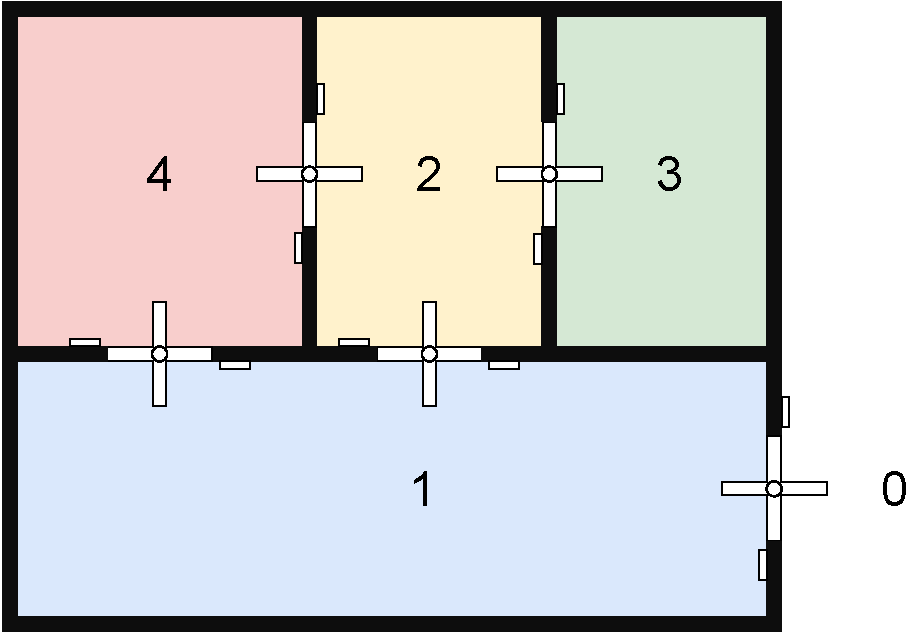
\includegraphics[width=1\linewidth]{facility}
			\caption{A top-down view of the facility with access areas marked
			with numbers. 0 denotes the ``outside'' access area.}
		\end{center}
	\end{figure}
	
	
	\subsection{System objectives}
	
	\begin{enumerate}
		\item \textbf{Access control} -- the administrator is able to configure
		which employees may enter which areas
		\item \textbf{Activity tracking and reports} -- the administrator is
		able to review the location of an employee as it changes with time and
		receive reports on how much time employees spend within an area
		\item \textbf{Access violation detection} -- the administrator is
		notified when an access violation occurs (e.g. the same ID card was
		used to enter the same room twice)
	\end{enumerate}
	
	\clearpage
	\section{Database entities and relations}
	
	\subsection{Schedule}
	
	Describes the work hours of an employee. Attributes include the start time
	and end time for each weekday. Used to detect when an employee is present
	in the building outside of work hours.
	
	\subsection{Employee}
	
	Basic entity describing an employee. Actions are associated with employees
	based on employee IDs encoded on ID cards.
	
	\subsubsection{Relation with schedule}
	
	Each employee has a schedule describing their work hours. Employees may
	share schedules. A schedule may be associated with no employees.
	
	\subsubsection{Relation with room}
	
	An employee may be permitted to enter zero or more rooms. A room may be
	entered by zero or more employees. Permissions may be temporary or
	permanent.
	
	\subsection{Room}
	
	Describes an access area employees may be permitted to enter.
	
	\subsection{Gate}
	
	Describes a connection between rooms. Together with the room entity it
	forms a graph describing the building.
	
	\subsubsection{Relation with room}
	
	A room may be connected to other rooms (or may contain an entrance to the
	building) through gates. Each gate connects two rooms.
	
	\subsection{Activity}
	
	Describes an action performed by an employee.
	
	\begin{center}
		\begin{tabular}{|c | c | p{10cm}|}
			\hline
			\textbf{Type} & \textbf{Name} & \textbf{Description} \\
			\hline
			0 & Unlocked & Unlocked a turnstile, but has yet to turn it. \\
			\hline
			1 & Passed & Turned the previously unlocked turnstile. \\
			\hline
			2 & Abandoned & The previously unlocked turnstile timed out and became locked again. \\
			\hline
		\end{tabular}
	\end{center}
	
	\subsubsection{Relation with employee, room and gate}
	
	The activity is associated with the employee who performed it. It is also
	described by the room where it happened and the gate that triggered it.
	
	\subsection{Violation}
	
	Describes an illegal action (security incident) performed by an employee.
	
	\begin{center}
		\begin{tabular}{|c | c | p{10cm}|}
			\hline
			\textbf{Type} & \textbf{Name} & \textbf{Description} \\
			\hline
			0 & Absent holder & The recorded location of the holder doesn't match the location of the gate. \\
			\hline
			1 & Unauthorized & The holder requested access to a room they are not permitted to enter. \\
			\hline
			2 & Overstayed & The holder was present in the facility outside of their work hours. \\
			\hline
			3 & Late entry & The holder attempted to enter the facility outside of their work hours. \\
			\hline
		\end{tabular}
	\end{center}
	
	\subsubsection{Relation with employee, room and gate}
	
	The violation is associated with the employee who performed it. The
	location and gate attributes apply if relevant.
	
	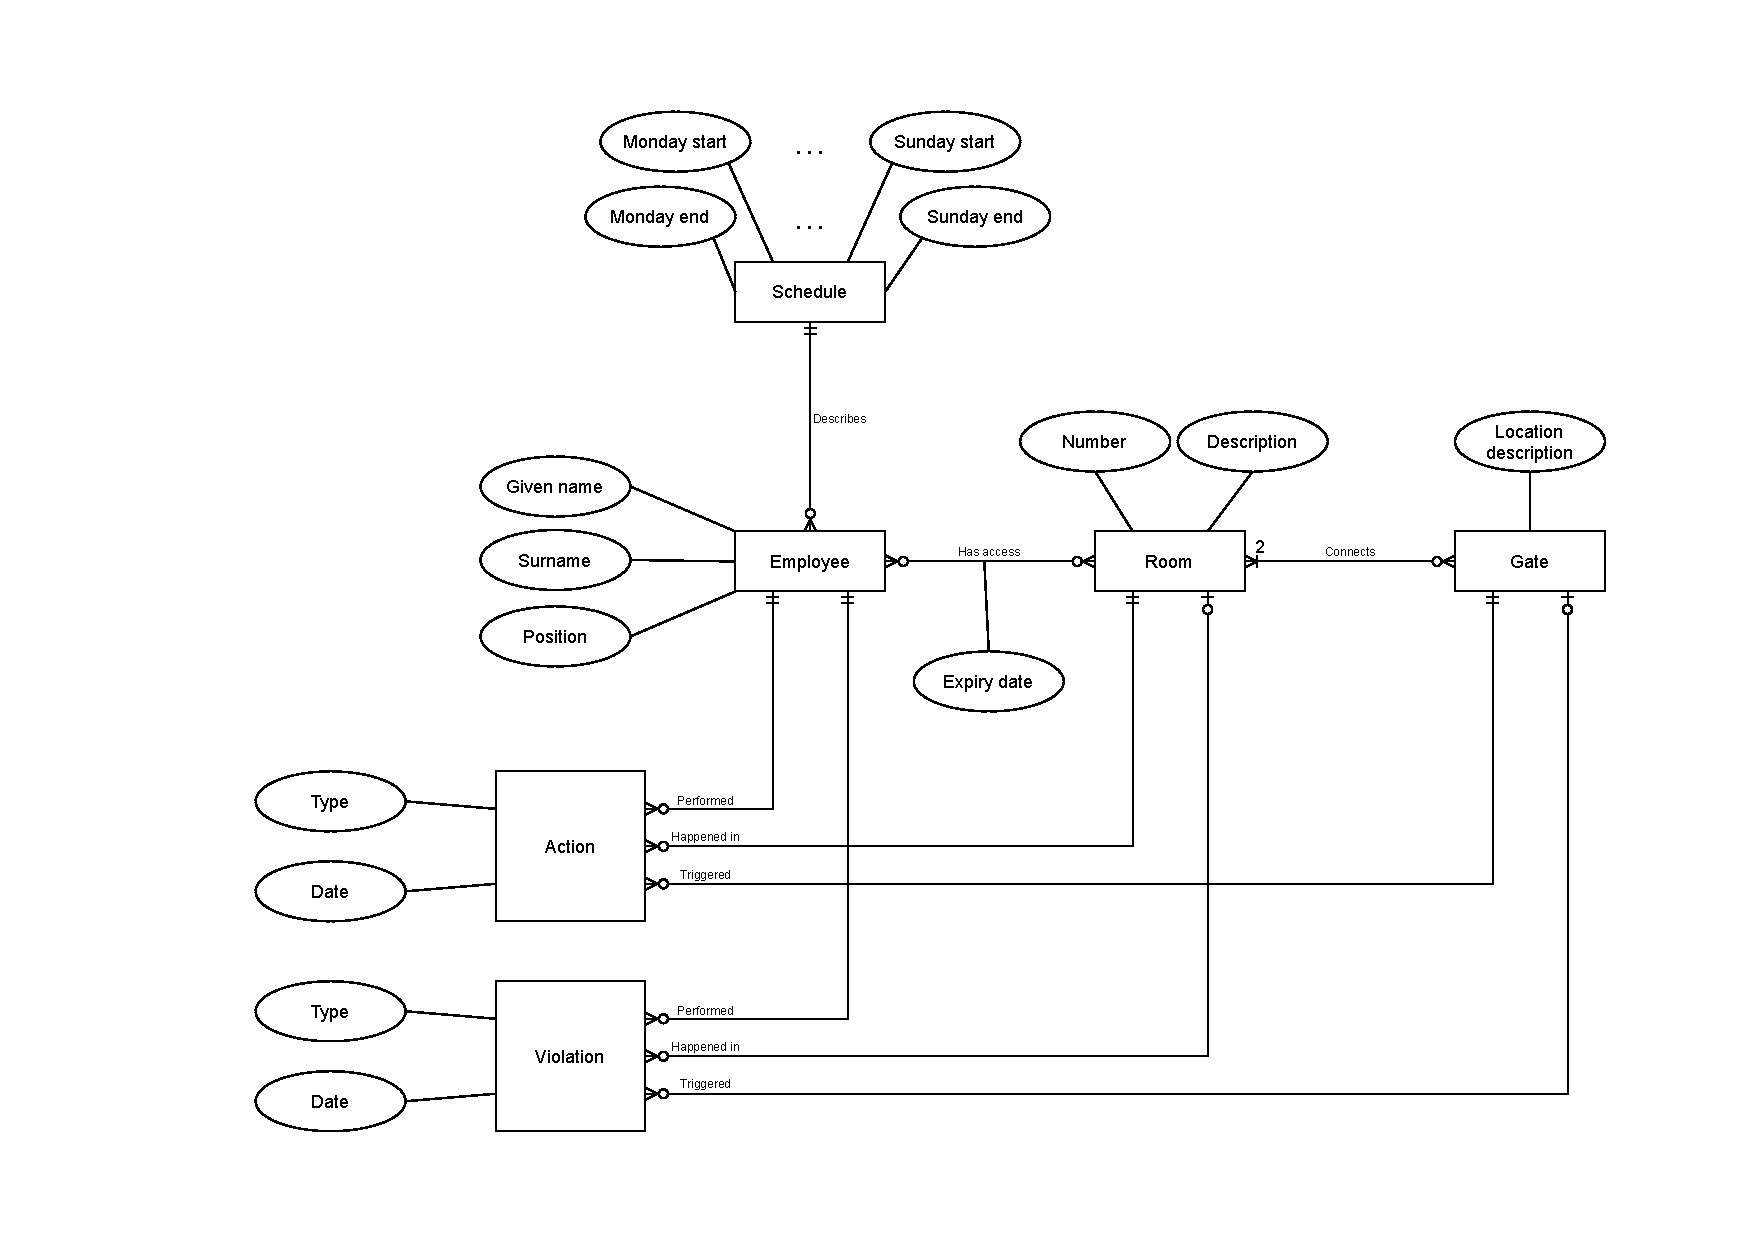
\includepdf{er}
	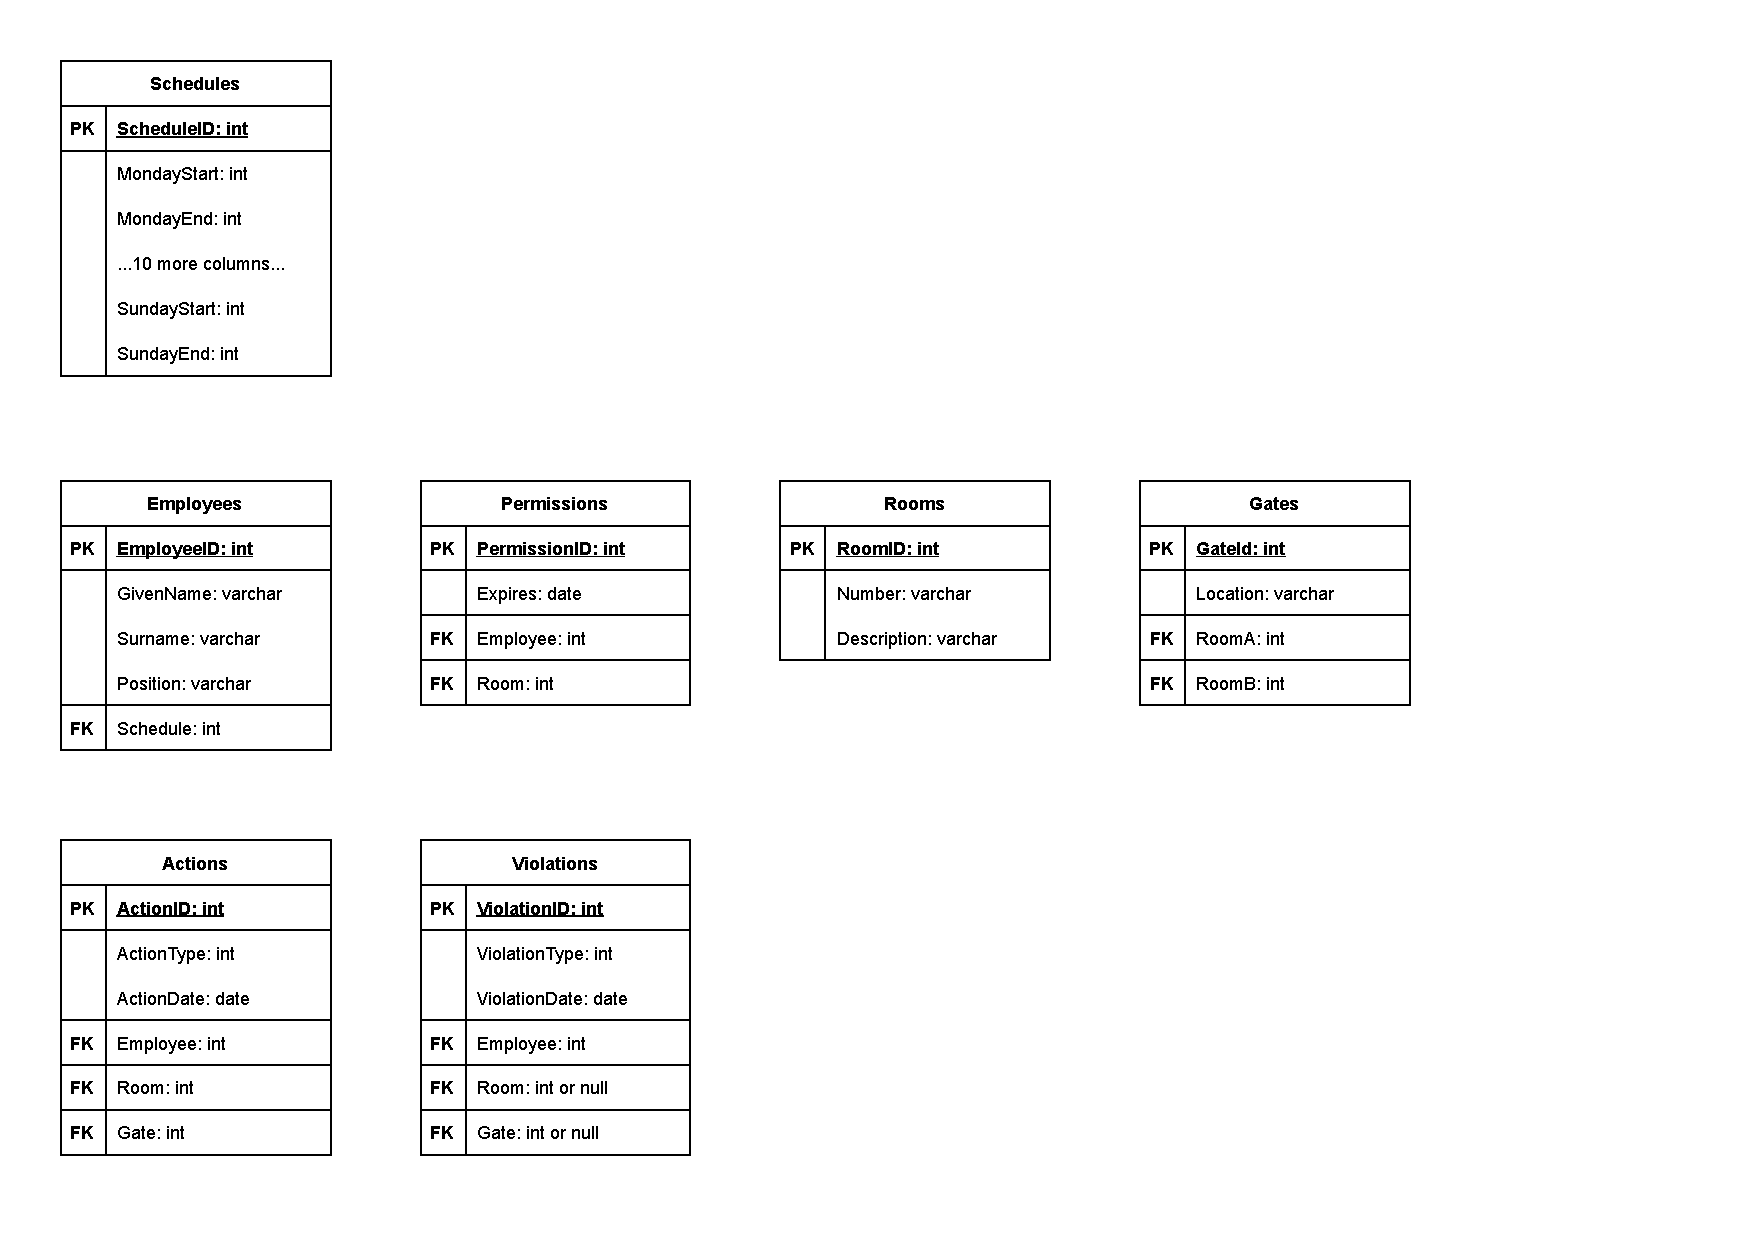
\includepdf{relational}
	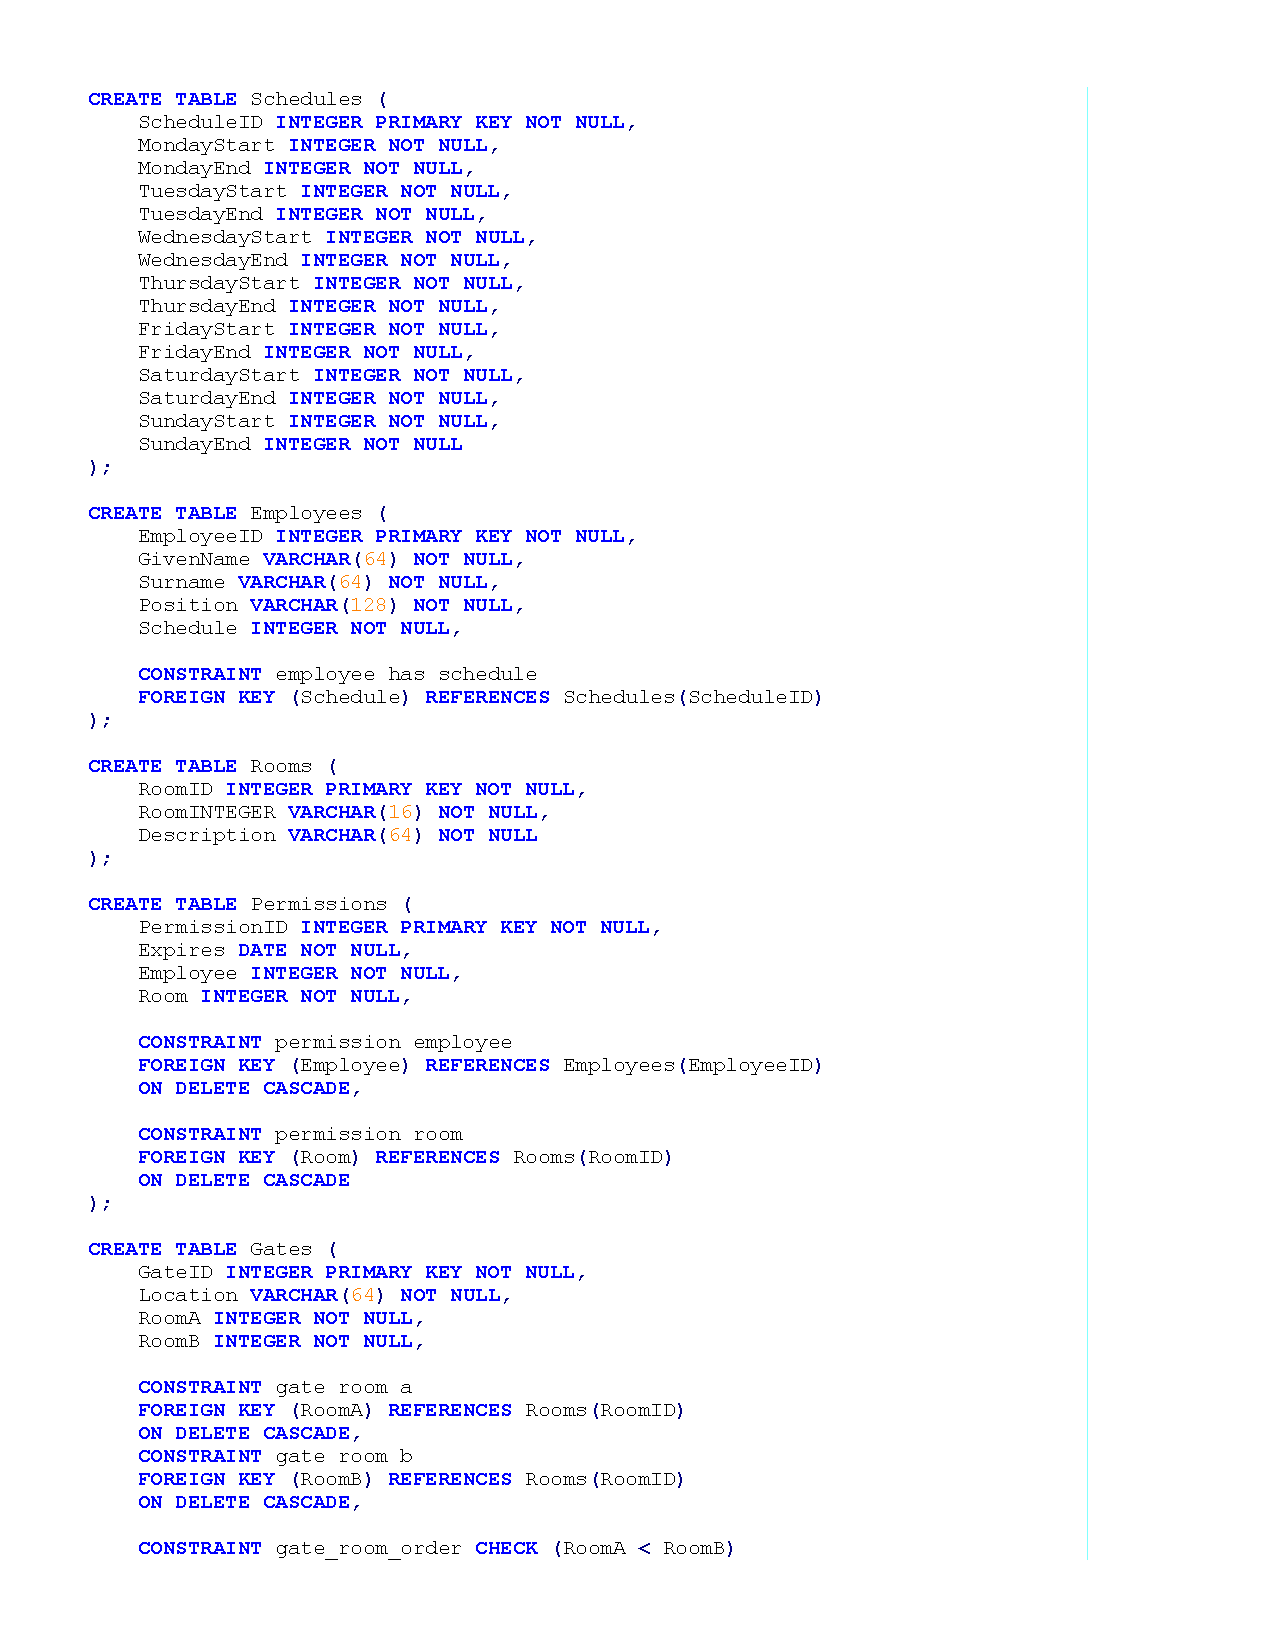
\includepdf[pages=-]{code}
	
\end{document}
